\documentclass[12pt,a4paper]{article}
\usepackage{cmap} % Makes the PDF copiable. See http://tex.stackexchange.com/a/64198/25761
\usepackage[T1]{fontenc}
\usepackage[brazil]{babel}
\usepackage[utf8]{inputenc}
\usepackage{amsmath}
\usepackage{amsfonts}
\usepackage{amssymb}
\usepackage{amsthm}
\usepackage{textcomp} % \degree
\usepackage{gensymb} % \degree
\usepackage[usenames,svgnames,dvipsnames]{xcolor}
\usepackage{hyperref}
\usepackage{multicol}
\usepackage{graphicx}
\usepackage[margin=2cm]{geometry}
\usepackage{systeme}
\usepackage{icomma}

\hypersetup{
    colorlinks = true,
    allcolors = {blue}
}

% TODO: Consider using exsheets
% http://linorg.usp.br/CTAN/macros/latex/contrib/exsheets/exsheets_en.pdf
%
% http://ctan.org/tex-archive/macros/latex/contrib/exercise/
% Options: answerdelayed,lastexercise,noanswer
\usepackage[answerdelayed,lastexercise]{exercise}

\addto\captionsbrazil{%
\def\listexercisename{Lista de exerc\'icios}%
\def\ExerciseName{Exerc\'icio}%
\def\AnswerName{Solu\c{c}\~ao do exerc\'icio}%
\def\ExerciseListName{Ex.}%
\def\AnswerListName{Solu\c{c}\~ao}%
\def\ExePartName{Parte}%
\def\ArticleOf{de\ }%
}

\renewcommand{\ExerciseHeaderTitle}{(\ExerciseTitle)\ }
\renewcommand{\ExerciseListHeader}{%\ExerciseHeaderDifficulty%
\textbf{%\ExerciseListName\
\ExerciseHeaderNB.\ %
%\ --- \
\ExerciseHeaderTitle}%
%\ExerciseHeaderOrigin
\ignorespaces}
\renewcommand{\AnswerListHeader}{\textbf{\ExerciseHeaderNB.\ (\AnswerListName)\ }}

\newcommand*\diff{\mathop{}\!\mathrm{d}}

\renewcommand{\theenumi}{\alph{enumi}}
\renewcommand\labelenumi{(\theenumi) }

\newcommand*\tipo{Prova III}
\newcommand*\turma{CCI192-04U}
\newcommand*\disciplina{ANN0001}
\newcommand*\eu{Helder G. G. de Lima}
\newcommand*\data{06/12/2024}

\author{\eu}
\title{\tipo - \disciplina}
\date{\data}

\begin{document}
\thispagestyle{empty}
\newgeometry{margin=2cm,bottom=0.5cm}
\begin{center}

\includegraphics[width=9.0cm]{marca} \\
\textbf{\tipo\ (\disciplina / \turma)} \\
Prof. \eu\footnote{
Este é um material de acesso livre distribuído sob os termos da licença \href{https://creativecommons.org/licenses/by-sa/4.0/deed.pt_BR}{Creative Commons BY-SA 4.0}}
\end{center}

\noindent Nome do(a) aluno(a): \underline{\hspace{9,7cm}} Data: \underline{\data}

%\section*{Instruções}
\begin{center}\fbox{
\begin{minipage}{14cm}
\begin{footnotesize}
\begin{itemize}
\renewcommand{\theenumi}{\Roman{enumi}}
\item Identifique-se em todas as folhas.
\item Mantenha o celular e os demais equipamentos eletrônicos desligados durante a prova.
\item Justifique cada resposta com cálculos ou argumentos baseados na teoria estudada.
\item Resolva $4$ das $5$ questões (deixe claro que questão não deverá ser corrigida).
\end{itemize}
\end{footnotesize}
\end{minipage}
}
\end{center}

%\section*{Questões}
\begin{ExerciseList}
\Exercise[title={2,5}] Encontre a função afim que melhor se ajusta, no sentido dos mínimos quadrados a $f(x) = x^2$ no intervalo $[-3, 3]$.
\Answer Se $y = \varphi(x) = a x + b$ é a função afim procurada, então $X = (a, b)^T$ é solução de $A X = B$, em que

\begin{minipage}{0.55\textwidth}

\[
   a_{11} = \int_{-3}^3 x^2 \diff{x} = \frac{3^3}{3} - \frac{-3^3}{3} = 18
\]
\[
   a_{12} = a_{21} = \int_{-3}^3 x \diff{x} = \frac{3^2}{2} - \frac{3^2}{2} = 0
\]
\[
   a_{22} = \int_{-3}^3 1 \diff{x} = 3 - (-3) = 6
\]
\[
   b_1 = \int_{-3}^3 x^3 \diff{x} = \frac{3^4}{4} - \frac{3^4}{4} = 0
\]
\[
   b_2 = \int_{-3}^3 x^2 \diff{x} = \frac{3^3}{3} - \frac{-3^3}{3} = 18
\]
Assim,
\[
   \begin{bmatrix}
      18 & 0 \\
      0 & 6
   \end{bmatrix}
   \cdot
   \begin{bmatrix}
      a \\
      b
   \end{bmatrix}
   =
   \begin{bmatrix}
      0 \\
      18
   \end{bmatrix}.
\]
Logo, $a = \frac{0}{18} = 0$, $b = \frac{18}{6} = 3$ e assim, $y = 0 x + 3$, isto é, $\boxed{y = 3}$.
    \end{minipage}\hfill
    \begin{minipage}{0.45\textwidth}
        \centering
        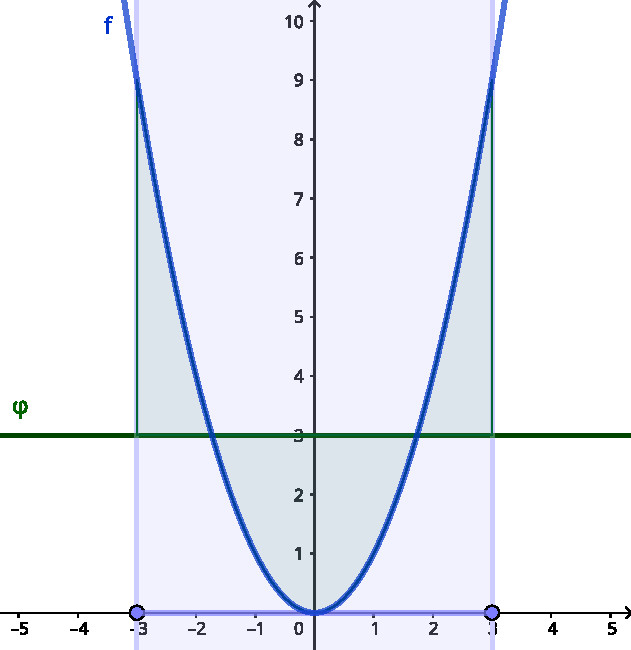
\includegraphics[width=0.9\textwidth]{img/mínimos-quadrados-contínuo.pdf}
    \end{minipage}



\Exercise[title={2,5}]
Utilize as raízes do polinômio de Chebyshev de grau dois, e (se necessário) uma transformação do intervalo, para construir um polinômio interpolador de grau menor ou igual a um para a função $f(x) = 3^x$ no intervalo $[0, 2]$. Use o polinômio obtido para aproximar $\sqrt[3]{3}$ ($=3^{1/3}$).
{\color{blue} \textit{(Arredonde os valores obtidos com 3 algarismos após a vírgula)}}
\Answer
O polinômio de Chebyshev de grau dois é dado por $T_2(x) = \cos(2\arccos(x)) = 2 x^2 - 1$ para $x \in [-1, 1]$, e suas raízes são $x_1 = \cos\left(\frac{1}{4}\pi\right) = \frac{\sqrt{2}}{2} \approx 0,707$ e $x_2 = \cos\left(\frac{3}{4}\pi\right) = -\frac{\sqrt{2}}{2} \approx -0,707$.

\begin{minipage}{0.75\textwidth}
Transformando o intervalo $[-1, 1]$ em $[0, 2]$ por meio de
\[
\tilde{x} = \frac{1}{2}[(2 - 0) x + (0 + 2)] = x + 1,
\]
obtemos $\tilde{x}_1 \approx 1,707$ e $\tilde{x}_2 \approx 0,293$. Por Lagrange, o polinômio que interpola $f(x) = 3^x$ nesses pontos é dado por:
\begin{align*}
    p(x)
    & = 3^{1,707} \left(\frac{x - 0,293}{1,707 - 0,293}\right)
    + 3^{0,293} \left(\frac{x - 1,707}{0,293 - 1,707}\right)\\
    & = 6,523 \left(\frac{x - 0,293}{1,414}\right)
    + 1,380 \left(\frac{x - 1,707}{-1,414}\right)\\
    & = 4,613(x - 0,293) - 0,976 (x - 1,707) \\
    & = 3,637x + 0,314.
\end{align*}

Portanto, $\sqrt[3]{3} = 3^{1/3} \approx 3,637 \cdot \left(\frac{1}{3}\right) + 0,314$, isto é, $\boxed{\sqrt[3]{3} \approx 1,526}$. Para fins de comparação, o valor exato, arredondado na quinto dígito decimal, é $\sqrt[3]{3} = 1,44225$.
\end{minipage}\hfill
\begin{minipage}{0.25\textwidth}
    \centering
    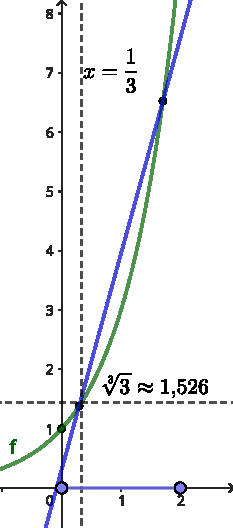
\includegraphics[width=0.8\textwidth]{img/interpolação-chebyshev.pdf}
\end{minipage}


\Exercise[title={2,5}] Mostre que a ordem de exatidão do método de Newton-Cotes aberto com dois pontos é igual a um (em outras palavras, ele é exato para funções afins mas não para funções quadráticas).
\Answer Para calcular a integral de uma função afim $f(x)$ em um intervalo $[a, b]$ pelo método de Newton-Cotes aberto com dois pontos, consideramos $h = \frac{b - a}{3}$, $x_0 = a + h$, $x_1 = a + 2h$ e aplicamos a fórmula \(\int_a^b f(x) \diff{x} \approx \frac{3h}{2} \cdot \left[ f(x_0) + f(x_1) \right]\). Para que a ordem de exatidão seja igual a um, é preciso que $k = 1$ seja o maior inteiro para o qual ocorre a igualdade
\[
\underbrace{\frac{3h}{2} \cdot \left[ x_0^k + x_1^k \right]}_{\text{Newton-Cotes aberta}}
= \underbrace{\frac{b^{k+1} - a^{k+1}}{k+1}}_{= \int_a^b x^k \diff{x}}.
\]

\textbf{Solução 1}:

\begin{itemize}
\item Para $k = 0$, temos $f(x) = x^0 = 1$ e:
\[
\frac{3h}{2} \cdot \left[ f(x_0) + f(x_1) \right]
= \frac{3\cdot \frac{b - a}{3}}{2} \cdot \left[ 1 + 1 \right]
= b - a
= \int_a^b 1 \diff{x}.
\]
\item Para $k = 1$, temos $f(x) = x^1 = x$ e:
\begin{align*}
\frac{3h}{2} \cdot \left[ f(x_0) + f(x_1) \right]
& = \frac{b - a}{2} \cdot \left[ x_0 + x_1 \right]
  = \frac{b - a}{2} \cdot \left[ \frac{2a + b}{3} + \frac{a + 2b}{3}\right] \\
& = \frac{b - a}{2} \cdot \left[ \frac{3a + 3b}{3}\right]
  = \frac{b - a}{2} \cdot \left[ a + b\right]
  = \frac{b^2 - a^2}{2}
  = \int_a^b x \diff{x}.
\end{align*}
\item Por outro lado, para $k = 2$, temos $f(x) = x^2$ e:
\begin{align*}
\frac{3h}{2} \cdot \left[ f(x_0) + f(x_1) \right]
& = \frac{b - a}{2} \cdot \left[ x_0^2 + x_1^2 \right]
= \frac{b - a}{2} \cdot \left[ \left(\frac{2a + b}{3}\right)^2 + \left(\frac{a + 2b}{3}\right)^2 \right] \\
& = \frac{b - a}{2} \cdot \left[ \frac{4a^2 + 4ab+b^2}{9} + \frac{a^2 + 4ab + 4b^2}{9} \right]\\
& = \frac{b - a}{2} \cdot \left[ \frac{5a^2 + 8ab + 5b^2}{9}\right]
\neq \frac{b^3 - a^3}{3}
= \int_a^b x^2 \diff{x}.
\end{align*}
\end{itemize}
Portanto, o maior valor de $k$ para o qual ocorre a igualdade é $\boxed{k = 1}$.

\textbf{Solução 2}: Como a fórmula do erro do método de Newton-Cotes aberto com dois pontos é 
\[
\int_a^b f(x) dx = \frac{3h}{2} \cdot \left[ f(x_0) + f(x_1) \right]
+ \underbrace{\frac{3h^3}{4} f^{(2)}(\xi)}_{\text{erro}},
\]
e $f^{(2)}(x) = 0$, para todo $x$, sempre que $f(x) = ax + b$, podemos concluir que o erro é zero nesses casos. Então basta verificar que a fórmula deixa de ser exata para funções quadráticas, como no caso $k=2$ da solução 1.


\Exercise[title={2,5}] Para cada item abaixo, indique se é verdadeiro (V) ou falso (F).

\emph{Observação 1:} Não é necessário justificar.

\emph{Observação 2:} Cada item marcado errado anula a pontuação de um item correto. Você pode deixar um item em branco para não perder nem ganhar pontos.

\begin{enumerate}
    \item {[0,9 ponto] \bf (\hspace{.7em})} A regra de quadratura gaussiana com um ponto é equivalente à regra do ponto médio.
    \item {[0,8 ponto] \bf (\hspace{.7em})} As regras de quadratura de 1/3 de Simpson e 3/8 de Simpson têm a mesma ordem de exatidão.
    \item {[0,8 ponto] \bf (\hspace{.7em})} No método de Runge-Kutta de ordem 4, o peso atribuído às inclinações é igual para todas as avaliações.
\end{enumerate}

\Answer
\begin{enumerate}
    \item \textbf{VERDADEIRO}: As fórmulas são idênticas.
    \item \textbf{VERDADEIRO}: Ambas têm ordem de exatidão $3$.
    \item \textbf{FALSO}: O peso é menor para as avaliações feitas nas extremidades do intervalo.
\end{enumerate}

\Exercise[title={2,5}] Considere o problema de valor inicial
\[
\begin{cases}
y^\prime(x) = -2 \cdot x \cdot y(x)\\
y(0) = 5
\end{cases}
\]
Aproxime o valor de $y(x)$ no intervalo $[0, 3]$ pelo método de \textbf{Euler implícito} com passo $h = 1$, e determine em qual dos pontos considerados ocorre o maior erro absoluto (em módulo) dessa aproximação, tendo em vista que a solução exata é $y(x)=5e^{-x^2}$.

{\color{blue} \textit{(Arredonde os valores obtidos com 3 algarismos após a vírgula)}}
\Answer Denotando $f(x,y) = -2 x y$ e $h = 1$, pode-se expressar a fórmula do método de Euler implícito da seguinte forma:
\[
y_{i + 1} = y_{i} + h f(x_{i + 1}, y_{i + 1})
= y_{i} + 1 \cdot ( -2 x_{i + 1} y_{i + 1} )
= y_{i} -2 x_{i + 1} y_{i + 1}
\]
que pode ser reescrita de forma equivalente como:
\[
y_{i + 1} = \frac{y_{i}}{1 + 2 x_{i + 1}} = \frac{y_{i}}{1 + 2 (x_i + 1)} = \frac{y_{i}}{2x_i + 3}.
\]

Disto resulta que os valores obtidos a cada passo são os seguintes:
\medskip
\begin{center}
\begin{tabular}{ccrcc}
\hline
$i$ & $x_i$ & $y_i$ & $y_{exato}(x_i)$ & $\varepsilon_i = y_i-y_{exato}(x_i)$ \\ \hline
$0$ & 0,000 & 5,000 & 5,000 & \phantom{-}0,000 \\
$1$ & 1,000 & 1,667 & 1,839 & -0,172 \\
$2$ & 2,000 & 0,333 & 0,092 & \phantom{-}0,241 \\
$3$ & 3,000 & 0,048 & 0,001 & \phantom{-}0,047 \\ \hline
\end{tabular}
\end{center}
\medskip
Assim, o maior erro absoluto em módulo é $|\varepsilon_2| = 0,241$, e ocorre em $\boxed{x_2 = 2}$.

\end{ExerciseList}

\vfill
\begin{center}
BOA PROVA E BOAS FÉRIAS!
\end{center}

\newpage
\restoregeometry
\section*{Respostas}
\shipoutAnswer
\end{document}
